\section{1174095 - Muhammad Dzihan Al-Banna}
\subsection{Soal Teori}
\begin{enumerate}

	\item Jelaskan kenapa kata-kata harus di lakukan vektorisasi. dilengkapi dengan ilustrasi atau gambar.
	\hfill\break
	Vektorisasi pada kata penting untuk mengetahui persentase kata yang sering muncul di setiap kalimat, hal ini berguna untuk menentukan kata kunci.

	\begin{figure}[H]
	\centering
		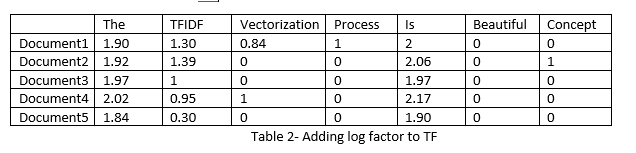
\includegraphics[width=4cm]{figures/1174095/tugas5/1.png}
		\caption{Teori 1}
	\end{figure}

	\item Jelaskan mengapa dimensi dari vektor dataset google bisa sampai 300. dilengkapi dengan ilustrasi atau gambar.

	\hfill\break 
	Setiap objek dalam dataset memiliki identitas khusus, misalnya ada 3 objek yang terdiri dari 3 dataset tersebut dilakukan perbandingan yang menghasilkan presentasi sebesar 75\%.
	\begin{figure}[H]
	\centering
		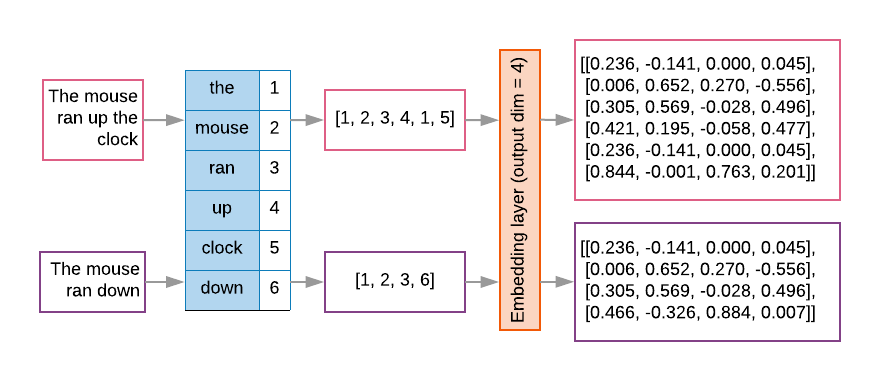
\includegraphics[width=4cm]{figures/1174095/tugas5/2.png}
		\caption{Teori 2}
	\end{figure}
	
	\item Jelaskan konsep vektorisasi untuk kata.dilengkapi dengan ilustrasi atau gambar.
	\hfill\break
	Konsep Vektorisasi kata sama seperti inputan kata-kata pada mesin pencari. Jadi kata tersebut akan dikeluarkan sebagai saran dari hasil pencarian sebelumnya yang saling berhubungan. misalnya orang sebelumnya pernah mencari stadion GBK digunakan sebagai venue Sea Games ajang sepakbola, maka apabila kamu mencari GBK, maka akan muncul juga SEA GAMES dan Sepak Bola sebagai saran pencarian.

	\begin{figure}[H]
	\centering
		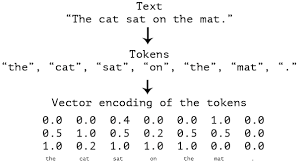
\includegraphics[width=4cm]{figures/1174095/tugas5/3.png}
		\caption{Teori 3}
	\end{figure}

	\item Jelaskan konsep vektorisasi untuk dokumen.dilengkapi dengan ilustrasi atau gambar.
	\hfill\break
	Sama halnya dengan vektorisasi kata, yang membedakan hanya pada proses awalnya. Untuk vektorisasi dokumen ini, mesin akan membaca semua kalimat yang terdapat pada dokumen tersebut, lalu kalimat yang terdapat pada dokumen akan di pecah menjadi kata-kata. Perhatikan gambar berikut : 

	\begin{figure}[H]
	\centering
		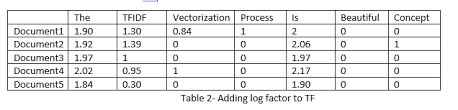
\includegraphics[width=4cm]{figures/1174095/tugas5/4.png}
		\caption{Teori 4}
	\end{figure}

	\item Jelaskan apa mean dan standar deviasi,dilengkapi dengan ilustrasi atau gambar.
	\hfill\break
	Mean adalah rata-rata yang didapatkan dari penjumlahan dari semua data kemudian dibagi dengan jumlah data. Sedangkan devasi adalah nilai statistik yang digunakan untuk menentukan distribusi data dan menentukan titik data individu dengan rata-rata nilai sampel

	\begin{figure}[H]
	\centering
		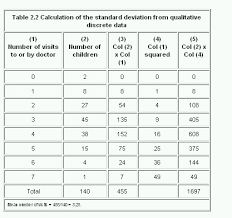
\includegraphics[width=4cm]{figures/1174095/tugas5/5.png}
		\caption{Teori 5}
	\end{figure}

	\item Jelaskan apa itu skip-gram,dilengkapi dengan ilustrasi atau gambar.
	\hfill\break
		Skip-gram dan vektorisasi kata hampir sama, dalam prakteknya skip gram mengambil kalimat lalu diolah untuk menemukan kata, kemudian kata tersebut akan diolah lagi menjadi suatu kalimat yang memiliki keterikatan dengan kata sebelumnya. 
	\begin{figure}[H]
	\centering
		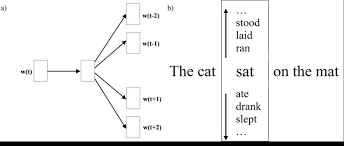
\includegraphics[width=4cm]{figures/1174095/tugas5/6.png}
		\caption{Teori 6}
	\end{figure}
\end{enumerate}


\subsection{Praktek Program}
\begin{enumerate}
	\item Soal 1
	\hfill\break
	\lstinputlisting[firstline=7, lastline=11]{src/1174095/tugas5/tugas5.py}
	Gensim adalah library yang digunakan untuk melakukan pemodelan dengan dataset yang telah ditentukan. Data diambil dari google dataset, dari 3 juta data yang tersedia di dalam google dataset tersebut, di kodingan diatas dibatasi hanya sampia 500000 data saja. Hasilnya sebagai berikut : 
	\begin{figure}[H]
	\centering
		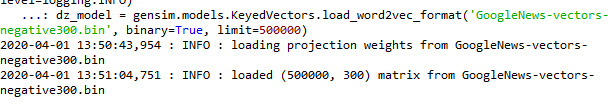
\includegraphics[width=4cm]{figures/1174095/tugas5/h1.PNG}
		\caption{Hasil Soal 1.}
	\end{figure}

	\hfill\break
	\lstinputlisting[firstline=13, lastline=14]{src/1174095/tugas5/tugas5.py}
	ini untuk menampilkan data hasil vektorisasi data dari kata love, hasilnya ialah sebagai berikut : 
	\begin{figure}[H]
	\centering
		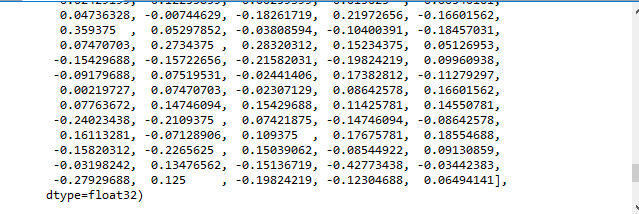
\includegraphics[width=4cm]{figures/1174095/tugas5/h2.PNG}
	\end{figure}

	\hfill\break
	\lstinputlisting[firstline=15, lastline=16]{src/1174095/tugas5/tugas5.py}
	ini untuk menampilkan data hasil vektorisasi data dari kata faith, hasilnya ialah sebagai berikut : 
	\begin{figure}[H]
	\centering
		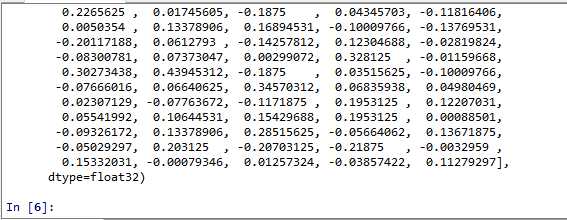
\includegraphics[width=4cm]{figures/1174095/tugas5/h3.PNG}
	\end{figure}

	\hfill\break
	\lstinputlisting[firstline=17, lastline=18]{src/1174095/tugas5/tugas5.py}
	ini untuk menampilkan data hasil vektorisasi data dari kata fall, hasilnya ialah sebagai berikut : 
	\begin{figure}[H]
	\centering
		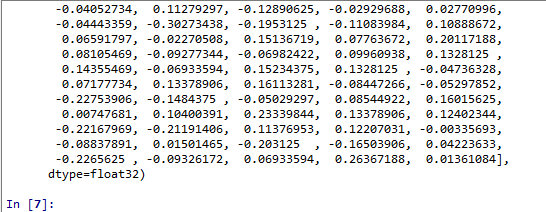
\includegraphics[width=4cm]{figures/1174095/tugas5/h4.PNG}
	\end{figure}

	\hfill\break
	\lstinputlisting[firstline=19, lastline=20]{src/1174095/tugas5/tugas5.py}
	ini untuk menampilkan data hasil vektorisasi data dari kata sick, hasilnya ialah sebagai berikut : 
	\begin{figure}[H]
	\centering
		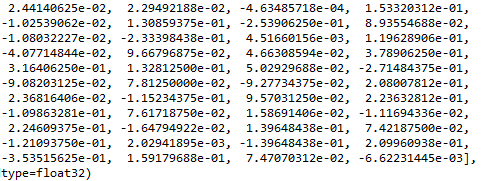
\includegraphics[width=4cm]{figures/1174095/tugas5/h5.PNG}
	\end{figure}

	\hfill\break
	\lstinputlisting[firstline=21, lastline=22]{src/1174095/tugas5/tugas5.py}
	ini untuk menampilkan data hasil vektorisasi data dari kata clear, hasilnya ialah sebagai berikut : 
	\begin{figure}[H]
	\centering
		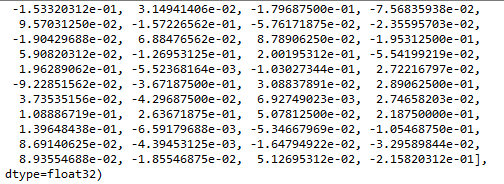
\includegraphics[width=4cm]{figures/1174095/tugas5/h6.PNG}
	\end{figure}

	\hfill\break
	\lstinputlisting[firstline=23, lastline=24]{src/1174095/tugas5/tugas5.py}
	ini untuk menampilkan data hasil vektorisasi data dari kata shine, hasilnya ialah sebagai berikut : 
	\begin{figure}[H]
	\centering
		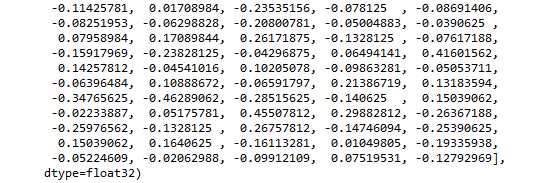
\includegraphics[width=4cm]{figures/1174095/tugas5/h7.PNG}
	\end{figure}

	\hfill\break
	\lstinputlisting[firstline=25, lastline=26]{src/1174095/tugas5/tugas5.py}
	ini untuk menampilkan data hasil vektorisasi data dari kata bag, hasilnya ialah sebagai berikut : 
	\begin{figure}[H]
	\centering
		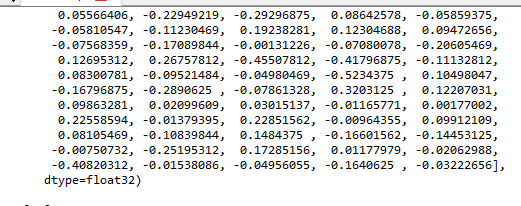
\includegraphics[width=4cm]{figures/1174095/tugas5/h8.PNG}
	\end{figure}

	\hfill\break
	\lstinputlisting[firstline=27, lastline=28]{src/1174095/tugas5/tugas5.py}
	ini untuk menampilkan data hasil vektorisasi data dari kata car, hasilnya ialah sebagai berikut : 
	\begin{figure}[H]
	\centering
		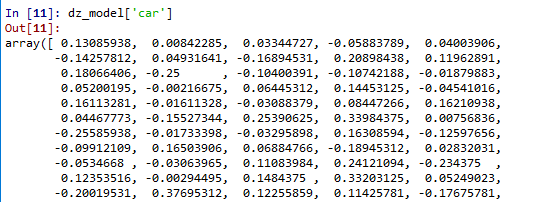
\includegraphics[width=4cm]{figures/1174095/tugas5/h9.PNG}
	\end{figure}

	\hfill\break
	\lstinputlisting[firstline=29, lastline=30]{src/1174095/tugas5/tugas5.py}
	ini untuk menampilkan data hasil vektorisasi data dari kata wash, hasilnya ialah sebagai berikut : 
	\begin{figure}[H]
	\centering
		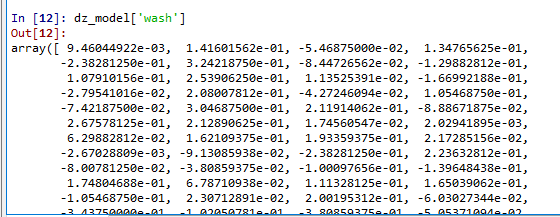
\includegraphics[width=4cm]{figures/1174095/tugas5/h10.PNG}
	\end{figure}

	\hfill\break
	\lstinputlisting[firstline=31, lastline=32]{src/1174095/tugas5/tugas5.py}
	ini untuk menampilkan data hasil vektorisasi data dari kata motor, hasilnya ialah sebagai berikut : 
	\begin{figure}[H]
	\centering
		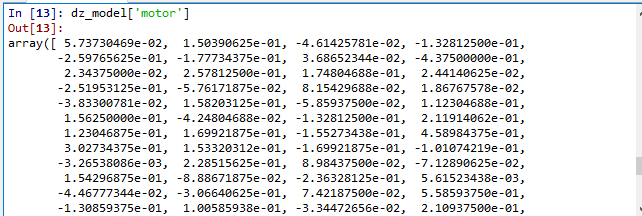
\includegraphics[width=4cm]{figures/1174095/tugas5/h11.PNG}
	\end{figure}

	\hfill\break
	\lstinputlisting[firstline=33, lastline=34]{src/1174095/tugas5/tugas5.py}
	ini untuk menampilkan data hasil vektorisasi data dari kata cycle, hasilnya ialah sebagai berikut : 
	\begin{figure}[H]
	\centering
		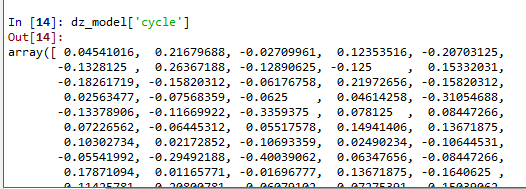
\includegraphics[width=4cm]{figures/1174095/tugas5/h12.PNG}
	\end{figure}


	\hfill\break
	\lstinputlisting[firstline=35, lastline=36]{src/1174095/tugas5/tugas5.py}
	Ini merupakan persentase dari perbandingan kata wash dan clear, persentase yang di dapat ialah 9 \% Hasil tersebut tidak terlalu baik, ialah sebagai berikut : 
	\begin{figure}[H]
	\centering
		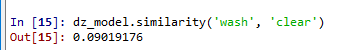
\includegraphics[width=4cm]{figures/1174095/tugas5/h13.PNG}
	\end{figure}

	\hfill\break
	\lstinputlisting[firstline=37, lastline=38]{src/1174095/tugas5/tugas5.py}
	Ini merupakan persentase dari perbandingan kata bag dan love, persentase yang di dapat ialah 7 \% Hasil tersebut tidak terlalu baik, ialah sebagai berikut 
	\begin{figure}[H]
	\centering
		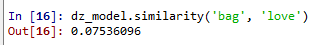
\includegraphics[width=4cm]{figures/1174095/tugas5/h14.PNG}
	\end{figure}

	\hfill\break
	\lstinputlisting[firstline=39, lastline=40]{src/1174095/tugas5/tugas5.py}
	Ini merupakan persentase dari perbandingan kata motor dan car, persentase yang di dapat ialah 48 \% Hasil tersebut cukup baik karena mesin dapat membedakan antara motor dan car, ialah sebagai berikut 
	\begin{figure}[H]
	\centering
		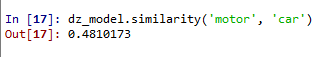
\includegraphics[width=4cm]{figures/1174095/tugas5/h15.PNG}
	\end{figure}

	\hfill\break
	\lstinputlisting[firstline=41, lastline=42]{src/1174095/tugas5/tugas5.py}
	Ini merupakan persentase dari perbandingan kata sick dan faith, persentase yang di dapat ialah 12 \% Hasil tersebut lumayan dibawah cukup, ialah sebagai berikut 
	\begin{figure}[H]
	\centering
		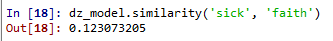
\includegraphics[width=4cm]{figures/1174095/tugas5/h16.PNG}
	\end{figure}

	\hfill\break
	\lstinputlisting[firstline=43, lastline=44]{src/1174095/tugas5/tugas5.py}
	Ini merupakan persentase dari perbandingan kata cycle dan shine, persentase yang di dapat ialah 9 \% Hasil tersebut buruk karena begitu sedikit persentase yang didapat, ialah sebagai berikut 
	\begin{figure}[H]
	\centering
		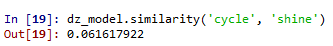
\includegraphics[width=4cm]{figures/1174095/tugas5/h17.PNG}
	\end{figure}


	\item Soal 2
	\hfill\break
	\lstinputlisting[firstline=46, lastline=54]{src/1174095/tugas5/tugas5.py}
	extract\_word digunakan sebagai string, pada kode di atas memakai import re. hasilnya sebagai berikut :
	\begin{figure}[H]
	\centering
		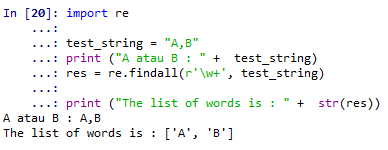
\includegraphics[width=4cm]{figures/1174095/tugas5/h18.PNG}
		\caption{Hasil Soal 2}
	\end{figure}

	\hfill\break
	\lstinputlisting[firstline=58, lastline=70]{src/1174095/tugas5/tugas5.py}
	Permutesentences digunakan untuk melerai atau memecah data, karena disitu terdapat random, sehinggan stringnya akan dipanggil secara acak. Hasilnya sebagai berikut :
	\begin{figure}[H]
	\centering
		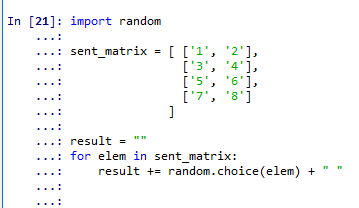
\includegraphics[width=4cm]{figures/1174095/tugas5/h19.PNG}
		\caption{Hasil Soal 2}
	\end{figure}
	
	\item Soal 3
	\hfill\break
	\lstinputlisting[firstline=74, lastline=94]{src/1174095/tugas5/tugas5.py}
	Fungsi dari gensim untuk membuat pemodelan tanpa pengawasan atau unsupervised. Doc2vec berfungsi untuk membandingkan bobot data yang terdapat pada dokumen lain apakah ada kata yang sama atau tidak. Tagged document berfungsi untuk memasukkan kata-kata setiap dokumennya untuk vektorisasi dan untuk membuat save model.
	\begin{figure}[H]
	\centering
		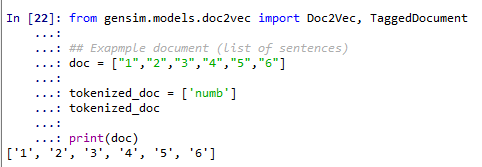
\includegraphics[width=4cm]{figures/1174095/tugas5/h20.PNG}
		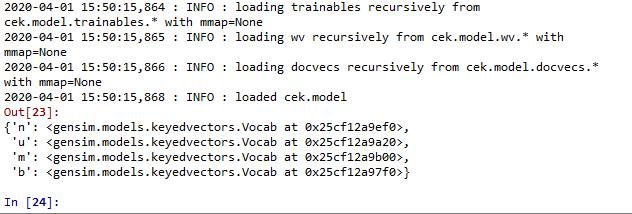
\includegraphics[width=4cm]{figures/1174095/tugas5/h21.PNG}
		
\includegraphics[width=4cm]{figures/1174095/tugas5/h22.PNG}
		\caption{Hasil Soal 3}
	\end{figure}

	\item Soal 4
	\hfill\break
	\lstinputlisting[firstline=98, lastline=109]{src/1174095/tugas5/tugas5.py}
	Disini kita memakai dataset dari aclImdb. Untuk menambahkan data training kita melakukan import library os, library os itu sendiri berfungsi untuk melakukan interaksi antara python dengan os laptop kita masing-masing, setelah itu kita buat variable unsup sentences. Selanjutnya pilih direktori tempat data kita disimpan. Selanjutnya itu untuk menyortir data yang terdapat pada folder aclImdb dan membaca file tersebut dengan ektensi .txt. Hasil dari code pertama tersebut ialah terdapatnya data hasil running dari folder aclImdb. Hasilnya adalah sebagai berikut :
	\begin{figure}[H]
	\centering
		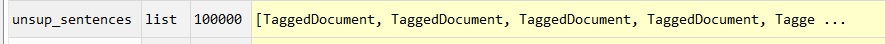
\includegraphics[width=4cm]{figures/1174095/tugas5/h23.PNG}
		\caption{Hasil Soal 4.}
	\end{figure}

	\item Soal 5
	\hfill\break
	\lstinputlisting[firstline=112, lastline=116]{src/1174095/tugas5/tugas5.py}
	Pada bagian ini, mute digunakan untuk mengacak data agar laptop ringan saat melakukan run. delete\_temporary digunakan untuk menghapus training yang sudah dilakukan sebelumny agar tidak membuat train selanjutnya berat di lapotp saat proses run. Hasilnya adalah sebagai berikut :
	\begin{figure}[H]

	\centering
		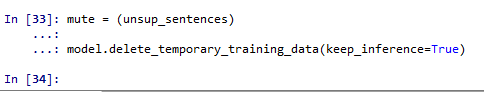
\includegraphics[width=4cm]{figures/1174095/tugas5/h24.PNG}
		\caption{Hasil Soal 5.}
	\end{figure}

	\item Soal 6
	\hfill\break
	\lstinputlisting[firstline=121, lastline=123]{src/1174095/tugas5/tugas5.py}
	Save data ini berfungsi untuk menyimpan file hasil dari proses pelatihan data sebelumnya, model tersebut dilakukan penyimpanan untuk memberikan keringanan pada ram agar saat kita akan melakukan pelatihan lagi, model tersebut tinggal di load saja tanpa harus melakukan pelatihan dari awal dan bisa menghemat waktu. Sedangkan untuk delete temporary training data ini berguna untuk menghapus data latihan yang sebelumnya sudah dilakukan dan disimpan, bertujuan untuk memberikan keringanan pada ram. Karena setelah melakukan proses pelatihan ram biasanya jadi tercekik sampai laptop jadi lag. Itulah fungsi dari delete temporary training data. Hasilnya adalah sebagai berikut :
	\begin{figure}[H]
	\centering
		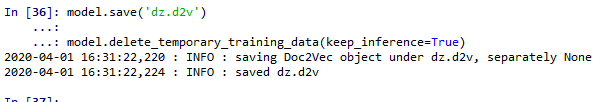
\includegraphics[width=4cm]{figures/1174095/tugas5/h25.PNG}
		\caption{Hasil Soal 6.}
	\end{figure}

	\item Soal 7
	\hfill\break
	\lstinputlisting[firstline=126, lastline=129]{src/1174095/tugas5/tugas5.py}
	Infer vector itu sendiri berguna untuk membandingkan kata yang tercantum dengan vektor yang mana pada dokumen yang sudah di load pada step sebelumnya. Selain itu infer vector juga untuk menghitung atau mengkalkulasikan vektor dari kata yang dicantumkan dari model yang telah kita buat. Alangkah baiknya kata yang dicantumkan itu lebih panjang lagi agar hasilnya bisa lebih baik lagi. Hasilnya adalah sebagai berikut :
	\begin{figure}[H]
	\centering
		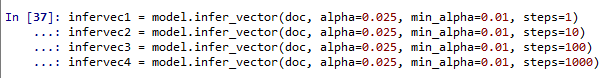
\includegraphics[width=4cm]{figures/1174095/tugas5/h26.PNG}
		\caption{Hasil Soal 7.}
	\end{figure}

	\item Soal 8
	\hfill\break
	\lstinputlisting[firstline=133, lastline=169]{src/1174095/tugas5/tugas5.py}
	Cosine similarity ini berfungsi untuk membandingkan vektorisasi data diantara kedua kata yang di inputkan, jika hasil presentase dari kedua kata tersebut lebih dari 50\% itu memiliki kemungkinan kata tersebut terdapat dalam 1 file. Namun jika kurang dari 50\% itu kemungkinan kata tersebut tidak terdapat dalam 1 file. Hasil yang didapatkan pada code tersebut hanya 0.8\% itu dikarenakan kata pertama dan kedua tidak memiliki kesamaan vektorisasi dan tidak terdapat pada salah satu dokumen. Hasilnya adalah sebagai berikut :
	\begin{figure}[H]
	\centering
		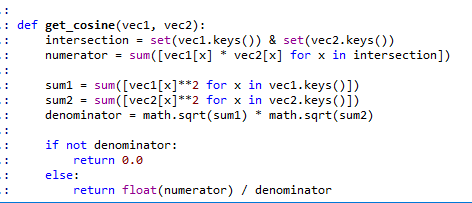
\includegraphics[width=4cm]{figures/1174095/tugas5/h27.PNG}
		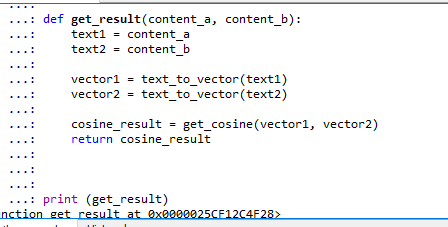
\includegraphics[width=4cm]{figures/1174095/tugas5/h28.PNG}
		\caption{Hasil Soal 8.}
	\end{figure}

	\item Soal 9
	\hfill\break
	\lstinputlisting[firstline=171, lastline=179]{src/1174095/tugas5/tugas5.py}
	Code tersebut akan melakukan perhitungan presentase dengan menggunakan cross validation dengan metode kneighborsClassifier. Memakai dataset iris, hasilnya adalah sebagai berikut :
	\begin{figure}[H]
	\centering
		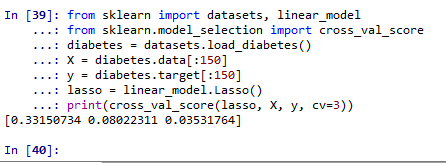
\includegraphics[width=4cm]{figures/1174095/tugas5/h29.PNG}
		\caption{Hasil Soal 9.}
	\end{figure}
\end{enumerate}

\subsection{Penanganan Error}
\begin{enumerate}
	\item ScreenShoot Error
	\begin{figure}[H]
		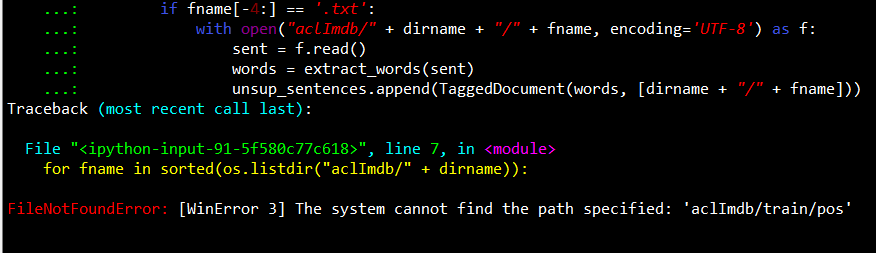
\includegraphics[width=4cm]{figures/1174095/tugas5/err1.PNG}
		\centering
		\caption{FileNotFoundError}
	\end{figure}
	\item Cara Penanganan Error
	\begin{itemize}
		\item FileNotFoundError
		\hfill\break
		Error terdapat pada dataset yang tidak terbaca, dengan ini saya mendownload dataset dari aclImdb, dan masalah error telah selesai.
	\end{itemize}
\end{enumerate}

\subsection{Bukti Tidak Plagiat}
\begin{figure}[H]
\centering
	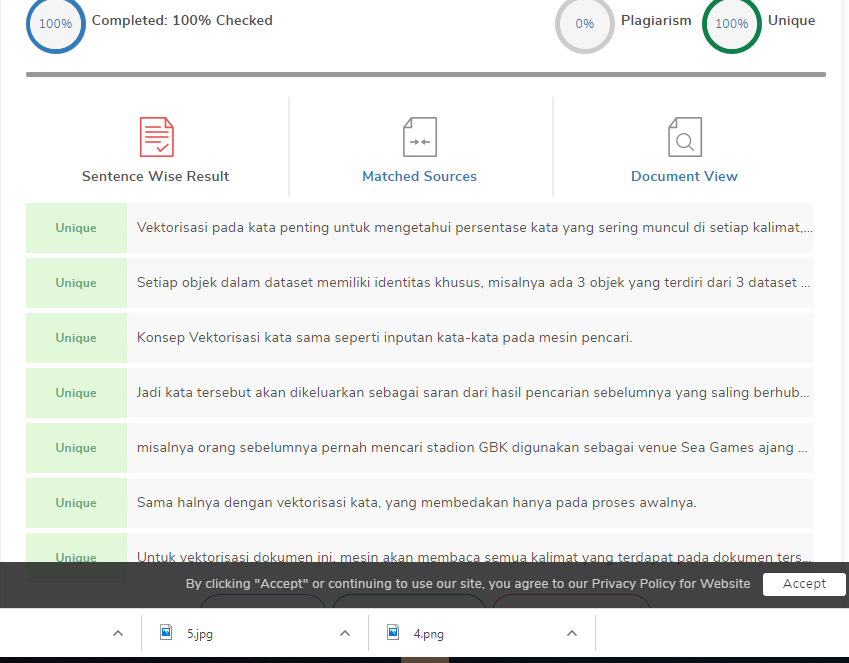
\includegraphics[width=4cm]{figures/1174095/tugas5/plag.PNG}
	\caption{Bukti Tidak Melakukan Plagiat Chapter 5}
\end{figure}

